\documentclass[xcolor=table]{beamer}

\usepackage[table,xcdraw]{xcolor}
\usepackage{graphicx}
\usepackage{textpos}
\usepackage{listings}
\usepackage{lstautogobble}

\usetheme{Madrid}
\useoutertheme{miniframes} % Alternatively: miniframes, infolines, split

% Setup the university's color pallette
\definecolor{UIUCorange}{RGB}{19, 41, 75} % UBC Blue (primary)
\definecolor{UIUCblue}{RGB}{232, 74, 39} % UBC Grey (secondary)

\definecolor{codegreen}{rgb}{0,0.6,0}
\definecolor{codegray}{rgb}{0.5,0.5,0.5}
\definecolor{codepurple}{rgb}{0.58,0,0.82}
\definecolor{backcolour}{rgb}{0.95,0.95,0.92}

\lstdefinestyle{python}{
  backgroundcolor=\color{backcolour},   
  commentstyle=\color{codegreen},
  keywordstyle=\color{magenta},
  numberstyle=\tiny\color{codegray},
  stringstyle=\color{codepurple},
  basicstyle=\ttfamily\footnotesize,
  breakatwhitespace=false,         
  belowskip=-0.5em,
  breaklines=true,                 
  captionpos=b,                    
  keepspaces=true,                 
  numbers=left,                    
  numbersep=5pt,                  
  showspaces=false,                
  showstringspaces=false,
  showtabs=false,                  
  tabsize=2
}

\lstset{style=python}

\AtBeginSection[]{
    \begin{frame}
        \vfill
        \centering
        \begin{beamercolorbox}[sep=8pt,center,shadow=true,rounded=true]{title}
            \usebeamerfont{title}\insertsectionhead\par%
        \end{beamercolorbox}
        \vfill
    \end{frame}
}

\setbeamercolor{palette primary}{bg=UIUCorange,fg=white}
\setbeamercolor{palette secondary}{bg=UIUCblue,fg=white}
\setbeamercolor{palette tertiary}{bg=UIUCblue,fg=white}
\setbeamercolor{palette quaternary}{bg=UIUCblue,fg=white}
\setbeamercolor{structure}{fg=UIUCorange} % itemize, enumerate, etc
\setbeamercolor{section in toc}{fg=UIUCblue} % TOC sections

\setbeamercolor{subsection in head/foot}{bg=UIUCorange,fg=UIUCblue}
\setbeamercolor{subsection in head/foot}{bg=UIUCorange,fg=UIUCblue}

\usepackage[utf8]{inputenc}
\usepackage{graphicx}

%\usepackage[shortlabels]{enumitem}

\title{\textbf{Topic 3: Sets and Dictionaries}}
\author{\textbf{David H Smith IV}}
\institute[\textbf{UIUC}]{\textbf{University of Illinois Urbana-Champaign}}
\date{\textbf{Wed, June 23 2021}}

\setbeamertemplate{title page}[default][colsep=-4bp,rounded=true]
\addtobeamertemplate{title page}{\vspace{3\baselineskip}}{}
\addtobeamertemplate{title page}{
  \begin{textblock*}{\paperwidth}(-1.0em, -1.2em)
    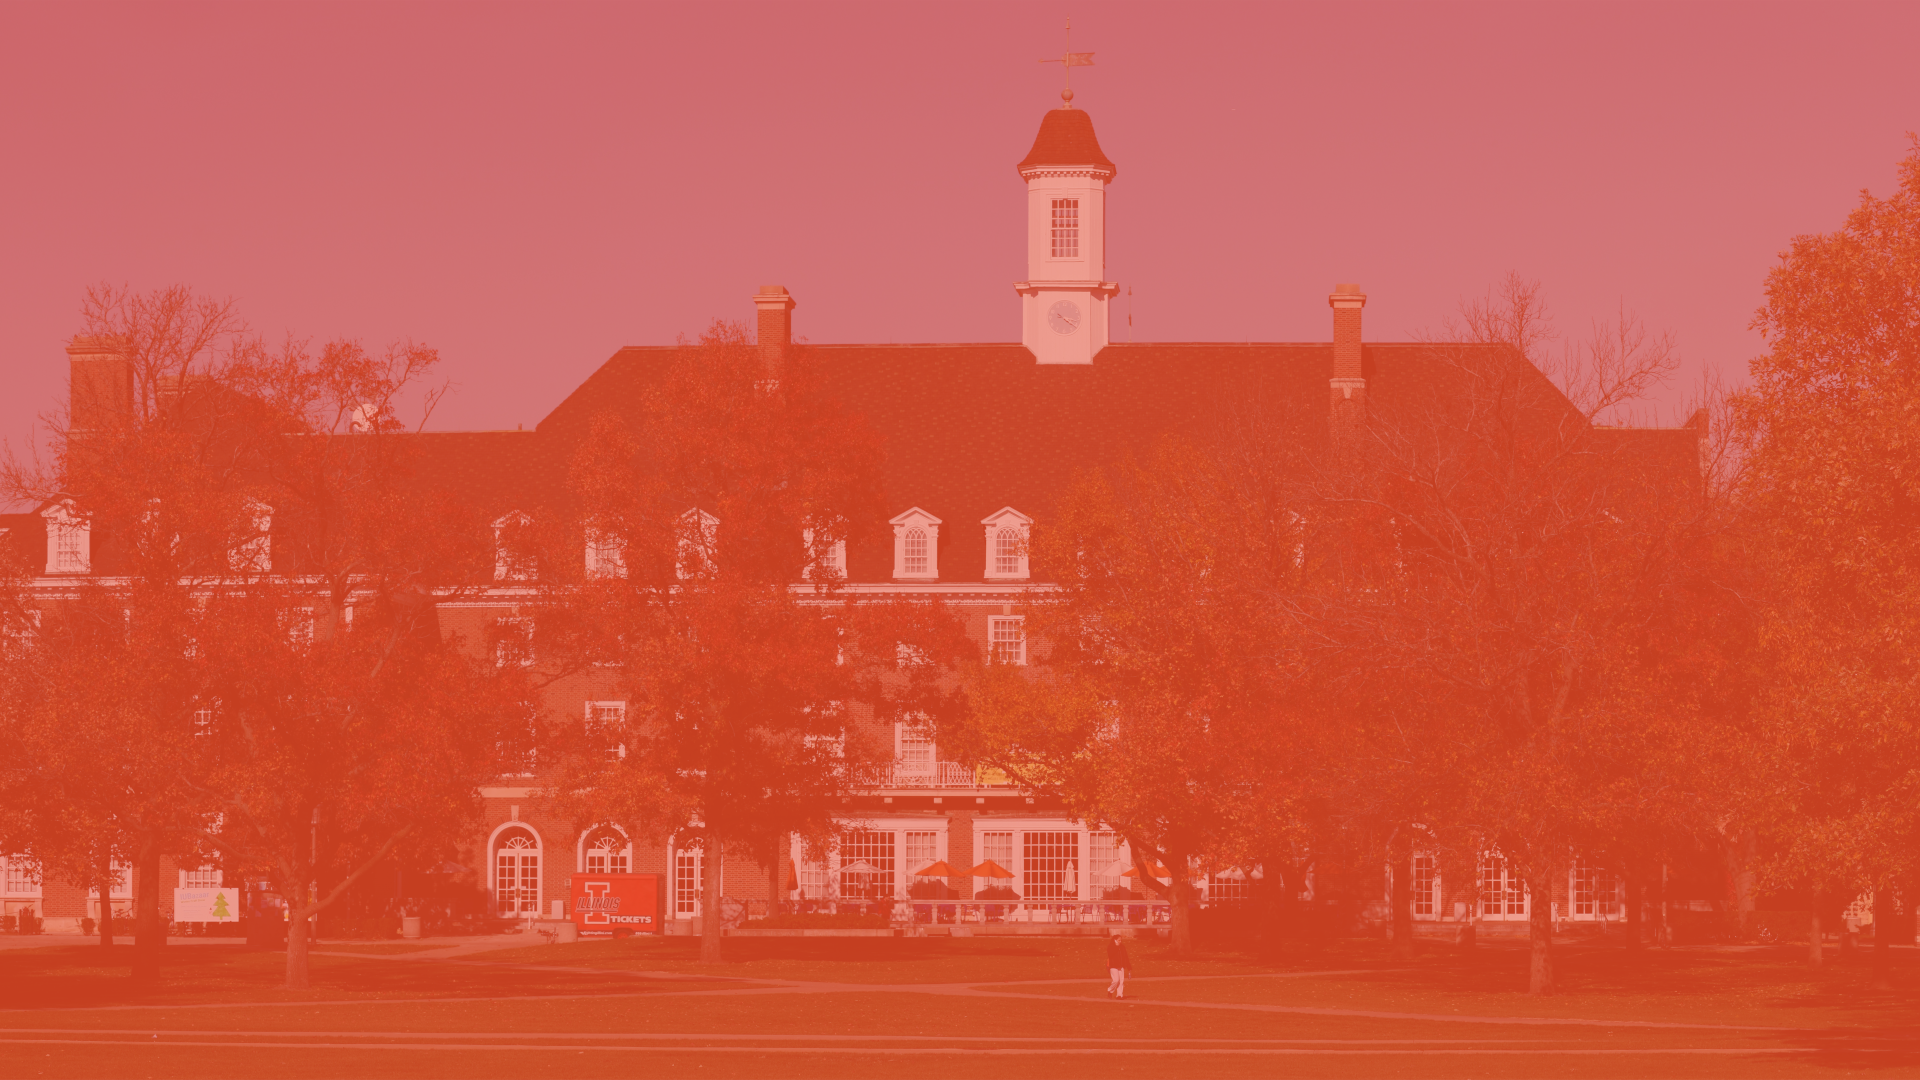
\includegraphics[width=\paperwidth, height=\paperheight]{imgs/uiuc.png}
  \end{textblock*} 
}{}

\begin{document}

\frame{\titlepage}

%
% Slide 8
%
\begin{frame}[fragile]
  \frametitle{Poll Question: Appending}
  What is the the value of \lstinline|x| after the following code runs?
  \begin{lstlisting}[language=Python, autogobble]
  x = [1, 2, 3]
  x = x.append(4)
  \end{lstlisting}
  \vfill
  \begin{enumerate}[A] 
    \item \lstinline|[1, 2, 3, 4]|
    \item AttributeError
    \item \lstinline|[1, 2, 3, [4]]|
    \item \lstinline|None|
  \end{enumerate}
\end{frame}

%
% Slide 8
%
\begin{frame}[fragile]
  \frametitle{Poll Question}
  What is the the type of \lstinline|x| after the following code runs?
  \begin{lstlisting}[language=Python, autogobble]
  x = (1, 2, 3)
  \end{lstlisting}
  \vfill
  \begin{enumerate}[A] 
    \item Set
    \item Dictionary
    \item List
    \item Tuple
  \end{enumerate}
\end{frame}

%
% Slide 8
%
\begin{frame}[fragile]
  \frametitle{Poll Question}
  What is the the type of \lstinline|x| after the following code runs?
  \begin{lstlisting}[language=Python, autogobble]
  x = [1, 2, 3]
  \end{lstlisting}
  \vfill
  \begin{enumerate}[A] 
    \item Set
    \item Dictionary
    \item List
    \item Tuple
  \end{enumerate}
\end{frame}

\section{Sets}

%
% Slide 10
%
\begin{frame}[fragile]
  \frametitle{Poll Question: Making Sets}
  Which of the following is an invalid way of making a set?
  \begin{enumerate}[A] 
    \item \lstinline|x = set(1, 2, 3)| 
    \item \lstinline|x = set([1, 2, 3])| 
    \item \lstinline|x = {1, 2, 3, 4}| 
    \item \lstinline|x = set()|
  \end{enumerate}
  \pause
  \vfill
  %\hline
  \vfill
  \begin{enumerate}
    \item \textbf{set()} \textrightarrow Creates either a new set by either accepting and converting another sequence type (e.g., list, tuple) or creates an empty list if it's not given anything.
    \item \textbf{set literal} \textrightarrow Written using the \lstinline|{}| with comma separated elements inside (e.g., \lstinline|{1, 2, 3}|).
  \end{enumerate}
\end{frame}

%
% This is a good place to remphasize the difference between inplace
% functions and functions that return a copy.
%
\begin{frame}[fragile]
  \frametitle{Poll Question: Set Tracing}
  What is the value of \lstinline|x| after this code has been run?
  \begin{lstlisting}[language=Python, autogobble]
  x = {1, 2, 3}
  y = {4, 5}
  x.union(y)
  \end{lstlisting}
  \vfill
  \begin{enumerate}[A] 
    \item None
    \item \lstinline|{1, 2, 3, 4, 5}|
    \item \lstinline|{}|
    \item \lstinline|{1, 2, 3}|
  \end{enumerate}
\end{frame}


%
% Slide 11
%
\begin{frame}[fragile]
  \frametitle{Poll Question: Updating Sets}
  \begin{lstlisting}[language=Python, autogobble]
  x = {1, 2, 3}
  y = set("aeiou")
  x.append(4)
  z = x + y
  print(z)
  \end{lstlisting}
  \vfill
  \begin{enumerate}[A] 
    \item \lstinline|{1, 2, 3, 4, "aeiou"}|
    \item \lstinline|{1, 2, 3, 4, "a", "e", "i", "o", "u"}|
    \item ValueError
    \item AttributeError
  \end{enumerate}
\end{frame}

%
% Slide 11
%
\begin{frame}[fragile]
  \frametitle{Poll Question: Updating Sets}
  \begin{lstlisting}[language=Python, autogobble]
  x = {1, 2, 3}
  y = set("aeiou")
  x.add(4)
  z = x + y
  \end{lstlisting}
  \vfill
  \begin{enumerate}[A] 
    \item \lstinline|{1, 2, 3, 4, "aeiou"}|
    \item \lstinline|{1, 2, 3, 4, "a", "e", "i", "o", "u"}|
    \item TypeError
    \item ValueError
  \end{enumerate}
\end{frame}

%
% Slide 11
%
\begin{frame}[fragile]
  \frametitle{Poll Question: Updating Sets}
  \begin{lstlisting}[language=Python, autogobble]
  x = {1, 2, 3}
  y = set("aeiou")
  x.add(4)
  z = x.union(y)
  \end{lstlisting}
  \vfill
  \begin{enumerate}[A] 
    \item \lstinline|{1, 2, 3, 4, "aeiou"}|
    \item \lstinline|{1, 2, 3, 4, "a", "e", "i", "o", "u"}|
  \end{enumerate}
\end{frame}

%
% This is a good place to remphasize the difference between inplace
% functions and functions that return a copy.
%
\begin{frame}[fragile]
  \frametitle{Poll Question: Set Tracing}
  How many total unique set objects are created throughout the duration of this
  codes runtime?
  \begin{lstlisting}[language=Python, autogobble]
  x = {1, 2, 3}
  y = {4, 5}
  x = x.union(y)
  z = set("test")
  x.update(z)
  \end{lstlisting}
  \vfill
  \begin{enumerate}[A] 
    \item 1
    \item 3
    \item 4
    \item 5
  \end{enumerate}
\end{frame}


%
% Slide 11
%
\begin{frame}[fragile]
  \frametitle{Poll Question: Set Tracing}
  What is the final value of set1 after the following code finish's executing?
  \begin{lstlisting}[language=Python, autogobble]
  set1 = {"hi", 2, 3}

  set2 = set([2, 3, 4])
  set2.add("hi")

  set1.update(set2)
  \end{lstlisting}
  \vfill
  \begin{enumerate}[A] 
    \item \lstinline|{"hi", 2, 3, 4}| %correct
    \item \lstinline|{"hi", 2, 2, 3, 3, 4}|
    \item \lstinline|{2, 3, 4}|
    \item AttributeError
  \end{enumerate}
\end{frame}

%
% Slide 9
%
\begin{frame}[fragile]
  \frametitle{Useful Set Functions}
  \begin{enumerate}
    \item \textbf{a.add(element)} \textrightarrow \ Adds a single element to a set.
    \item \textbf{a.update(b)} \textrightarrow \ Adds all the elements from \lstinline|b| to \lstinline|a|. This function does not return anything.
    \item \textbf{c = a.union(b)} \textrightarrow \ Creates a \textbf{new} set containing all of the elements from \lstinline|a| and \lstinline|b| and stores it in \lstinline|c|.
    \item \textbf{c = a.intersection(b)} \textrightarrow \ Creates a \textbf{new} set containing the intersection of \lstinline|a| and \lstinline|b| and stores it in \lstinline|c|.
    \item \textbf{c = a.difference(b)} \textrightarrow \ Creates a \textbf{new} set containing the intersection of \lstinline|a| and \lstinline|b| and stores it in \lstinline|c|.
  \end{enumerate}
\end{frame}



\section{Dictionaries}


%
% Slide 13
%
\begin{frame}[fragile]
  \frametitle{Poll Question: Accessing Element in Dictionary}
  What is the resulting value of \lstinline|d| after the following code is executed?
  \begin{lstlisting}[language=Python, autogobble]
  d = {}
  d["foo"] = 1
  d["bar"] = 2
  d["baz"] = 3
  \end{lstlisting}
  \vfill
  \begin{enumerate}[A] 
    \item SyntaxError
    \item TypeError
    \item \lstinline|{"foo": 1, "bar": 2, "baz": 3}|
    \item \lstinline|{"baz": 3}|
  \end{enumerate}
\end{frame}


%
%
%
\begin{frame}[fragile]
  \frametitle{Poll Question: Accessing Element in Dictionary}
  Given the following dictionary, what is the correct way to access the value with the key \lstinline|"foo"|?
  \begin{lstlisting}[language=Python, autogobble]
  d = {"foo": 5, "bar": 10, "baz": 2}
  \end{lstlisting}
  \vfill
  \begin{enumerate}[A] 
    \item You can't. Dictionaries are unordered.
    \item \lstinline|d[0]|
    \item \lstinline|d("foo")|
    \item \lstinline|d["foo"]| %correct
  \end{enumerate}
\end{frame}


%
% Reference similarity between dictionaries and lists 
%
\begin{frame}[fragile]
  \frametitle{Poll Question: Accessing Element in Dictionary}
  What is the resulting value of \lstinline|d| after the following code is executed?
  \begin{lstlisting}[language=Python, autogobble]
  d = {"foo": 5, "bar": 10, "baz": 2}
  d["foo"] = 2
  del d["baz"] 
  \end{lstlisting}
  \vfill
  \begin{enumerate}[A] 
    \item You can't. Dictionaries are unordered.
    \item \lstinline|{"foo": 2, "bar": 10}|
    \item \lstinline|{"foo": 5, "foo": 2, "bar": 10, "baz": 2}|
    \item \lstinline|{"foo": 5, "foo": 2, "bar": 10}|
    \item \lstinline|{"foo": 2, "bar": 10, "baz": }|
  \end{enumerate}
\end{frame}

%
% Reference similarity between dictionaries and lists 
%
\begin{frame}[fragile]
  \frametitle{New Dictionary Functions}
  What is the resulting value of \lstinline|d| and \lstinline|x| after the following code is executed?
  \begin{lstlisting}[language=Python, autogobble]
  d = {"Washington": 5, "California": 10, "Oregon": 2}
  x = d.pop("Washington")
  \end{lstlisting}
  \vfill
  \begin{enumerate}[A] 
    \item AttributeError
    \item \lstinline|d={"Washington": 5, "California": 10, "Oregon": 2}| and \lstinline|x=5|
    \item \lstinline|d={"Washington": 5, "California": 10, "Oregon": 2}| and  \lstinline|x="Washington"|
    \item \lstinline|d={"California": 10, "Oregon": 2}| and \lstinline|x=5|
    \item \lstinline|d={"California": 10, "Oregon": 2}| and \lstinline|x={"Washington": 5}|
  \end{enumerate}
\end{frame}

%
% Reference similarity between dictionaries and lists 
%
\begin{frame}[fragile]
  \frametitle{New Dictionary Functions}
  What is the resulting value of \lstinline|x| after the following code is executed?
  \begin{lstlisting}[language=Python, autogobble]
    x = {"hello": 5, "world": 10}
    y = {"world": 11, "!": 12}
    x.update(y)
  \end{lstlisting}
  \vfill
  \begin{enumerate}[A] 
    \item AttributeError
    \item \lstinline|{'hello': 5, 'world': 10, '!': 12}| 
    \item \lstinline|{'hello': 5, 'world': 11, '!': 12}| 
    \item \lstinline|{'hello': 5, 'world': 12, '!': 12}| 
  \end{enumerate}
\end{frame}

%
% Slide 13
%
\begin{frame}[fragile]
  \frametitle{Dictionaries}
  \begin{enumerate}[A] 
    \item Consists of key:value pairs.
    \item \lstinline|{key1:value1, key2:value2, key3:value3}|
    \item All keys must be unique.
    \item Access method is similar to lists but we use keys instead of indices (i.e., list[0] vs dict[key]).
  \end{enumerate}
\end{frame}


\section{String Formatting}

\begin{frame}[fragile]
  \frametitle{Poll Question: String Formatting}
  What is the value of x after the following code executes:
  \begin{lstlisting}[language=Python, autogobble] 
  x = "{1} {0} {1}".format("S", "O", "Y")
  \end{lstlisting}
  \vfill
  \begin{enumerate}[A] 
    \item \lstinline|"S O Y"|
    \item \lstinline|"SOY"|
    \item \lstinline|"O S O"| %correct
    \item \lstinline|"Y O Y"|
    \item \lstinline|"OSO"|
  \end{enumerate}
\end{frame}

\begin{frame}[fragile]
  \frametitle{Poll Question: String Formatting}
  What is the value of x after the following code executes:
  \begin{lstlisting}[language=Python, autogobble] 
  import math
  x = "{1:.3f} {0:.2f} {2:.4f}".format(math.pi, math.e, math.tau)
  \end{lstlisting}
  \vfill
  \begin{enumerate}[A] 
    \item SyntaxError
    \item \lstinline|"2.718 3.14 6.2832"|
    \item \lstinline|"2.71 3.1 6.283"| 
    \item \lstinline|"3.142 2.72 6.2832"|
  \end{enumerate}
\end{frame}

\section{Data Types Conclusion}

%
%
%
\begin{frame}[fragile]
  \frametitle{Poll Question: Set Tracing}
  What is the type of \lstinline|x|?
  \begin{lstlisting}[language=Python, autogobble]
  x = {1, 2, 3}
  \end{lstlisting}
  \vfill
  \begin{enumerate}[A] 
    \item 1
    \item 3
    \item 4
    \item 5
  \end{enumerate}
\end{frame}


%
% Slide 9
%
\begin{frame}[fragile]
  \frametitle{}
  Syntax for creation:
  \begin{enumerate}
    \item \textbf{\{\}} \textrightarrow \ For creating sets \textbf{only if there are elements in between}.
    \item \textbf{\{\}} \textrightarrow \ Creating dictionaries when left blank.
  \end{enumerate}
  \vfill
  Conversion/creation functions:
  \begin{enumerate}
    \item \textbf{set()} \textrightarrow \ Either converts a sequence type to a set or creates a blank set.
    \item \textbf{dict()} \ Creates a blank dict or converts a list of tuples (where each tuple has \textbf{exactly} two elements) to a dictionary.
  \end{enumerate}
\end{frame}


%
% Slide 9
%
\begin{frame}[fragile]
  \frametitle{Order and Mutability}
  % Please add the following required packages to your document preamble:
  \begin{table}[]
    \begin{tabular}{l|l|l}
      \hline
      \multicolumn{1}{c|}{}       & \multicolumn{1}{c|}{Ordered}                  & \multicolumn{1}{c}{Mutable}                  \\ \hline
      \multicolumn{1}{c|}{String} & \multicolumn{1}{c|}{\cellcolor[HTML]{34FF34}} & \multicolumn{1}{c}{\cellcolor[HTML]{FE0000}} \\ \hline
      List                        & \cellcolor[HTML]{34FF34}                      & \cellcolor[HTML]{34FF34}                     \\ \hline
      Tuple                       & \cellcolor[HTML]{34FF34}                      & \cellcolor[HTML]{FE0000}                     \\ \hline
      Set                         & \cellcolor[HTML]{FE0000}                      & \cellcolor[HTML]{34FF34}                     \\ \hline
      Dict                        & \cellcolor[HTML]{FE0000}                      & \cellcolor[HTML]{34FF34}                     \\ \hline
    \end{tabular}
  \end{table}
  \pause
  This is a lot to remember. So memorize it through practice rather than through standard memorization. 
\end{frame}



\section{Final Reminders}

\begin{frame}
  \frametitle{Announcements}
  \begin{enumerate}
    \item Usual mix of post-readings, participation, and homework are due tomorrow.
    \item Lab is due Sunday along with the zyBook challenge activities.
  \end{enumerate}
\end{frame}



\end{document}
